\documentclass[a4paper]{article}

\usepackage[T1]{fontenc}
\usepackage[utf8]{inputenc}
\usepackage{lmodern}
\usepackage{mathtools}
\usepackage{palatino}
\usepackage{amssymb}
\usepackage{amsthm}
\usepackage{graphicx}
\usepackage{subcaption}
\usepackage{booktabs}
\usepackage{tabulary}
\usepackage{rotating}
\usepackage[margin=2cm]{geometry}
\usepackage{listings}
\usepackage[ruled,vlined]{algorithm2e}
\usepackage{hyperref}
\usepackage[nameinlink,capitalise]{cleveref}
\usepackage{todonotes}
\usepackage[round,sort&compress]{natbib}
\usepackage[acronym,smallcaps,nowarn,section,nogroupskip,nonumberlist]{glossaries}

%% Custom package setup
% graphics
\graphicspath{{images/}}
% bib
\bibliographystyle{unsrtnat}
% abbreviations
\glsdisablehyper{}
\newacronym{VAE}{vae}{variational auto-encoder}
\newacronym{KL}{kl}{Kullback-Leibler}
\newacronym{SGD}{sgd}{stochastic gradient descent}
\newacronym{SGA}{sga}{stochastic gradient ascent}
\newacronym{CDAE}{cdae}{coordinate descent auto-encoder}
\newacronym{ELBO}{elbo}{evidence lower bound}
\newacronym{EUBO}{eubo}{evidence upper bound}
% cleveref
\crefname{algorithm}{Algorithm}{Algorithms}
\crefname{equation}{Equation}{Equations}
\crefname{figure}{Figure}{Figure}
% todonotes
\presetkeys{todonotes}{%
  backgroundcolor=blue!10!white,
  linecolor=blue!10!white,
  bordercolor=blue!10!white
}{}
% misc
\usepackage[parfill]{parskip}   % skip line instead of indent

% http://tex.stackexchange.com/questions/112580/rescaling-a-math-symbol
\usepackage{scalerel}
\usepackage{mleftright}
\usepackage{dsfont}
\newcommand\scalesym[2]{\hstretch{#1}{\vstretch{#1}{#2}}}

% -- operators
\DeclareMathOperator{\E}{{}\mathbb{E}}
\DeclareMathOperator{\1}{{}\mathds{1}}
\DeclareMathOperator{\DKL}{{}\mathbb{D}_{\text{\scalebox{0.75}{KL}}}}
\DeclareMathOperator*{\argmin}{arg\,min} % * allows typesetting beneath
\DeclareMathOperator*{\argmax}{arg\,max} % * allows typesetting beneath
\DeclareMathOperator*{\maximize}{maximize}
\DeclareMathOperator*{\minimize}{minimize}
\DeclareMathOperator{\ELBO}{\acrshort{ELBO}}
\DeclareMathOperator{\EUBO}{\acrshort{EUBO}}

% -- helpers
\renewcommand{\vec}[1]{\boldsymbol{\mathbf{#1}}}
\renewcommand{\to}{\ensuremath{\rightarrow}}              % add ensure math
\newcommand{\from}{\ensuremath{\leftarrow}}
\newcommand{\given}{\mid}
\renewcommand{\~}{\,\scalesym{0.7}{\thicksim}\,}          % what is this renewing?
\newcommand{\grpP}[1]{\ensuremath{\mleft( #1 \mright)}}   % parens   ()
\newcommand{\grpB}[1]{\ensuremath{\mleft\{ #1 \mright\}}} % braces   {}
\newcommand{\grpS}[1]{\ensuremath{\mleft[ #1 \mright]}}   % brackets []
\newcommand{\fnP}[2]{\ensuremath{#1 \grpP{#2}}}           % parens   ()
\newcommand{\fnB}[2]{\ensuremath{#1 \grpB{#2}}}           % braces   {}
\newcommand{\fnS}[2]{\ensuremath{#1 \grpS{#2}}}           % brackets []
\newcommand{\KL}[2]{\fnP{\DKL}{#1 \,\|\; #2}}             % kl divergence
\newcommand{\Ex}[2][]{\fnS{\E_{#1}}{#2}}                  % expectation

% -- special
\newcommand{\p}[2][]{\fnP{p_{#1}}{#2}}
\newcommand{\q}[2][]{\fnP{q_{#1}}{#2}}

%%% Local Variables:
%%% mode: latex
%%% TeX-master: "notes"
%%% End:


\title{Notes: Coordinate Descent Auto-Encoder}
\author{Tuan Anh and Sid}
\date{\today}

\begin{document}
\maketitle

\listoftodos

% !tex root=./notes.tex

\section{Introduction}
\label{sec:introduction}

We're trying to simultaneously
\begin{itemize}
    \item learn the forward generative model, and
    \item amortize inference
\end{itemize}
in a way that doesn't require the reparameterization trick~\citep{kingma2014auto,rezende2014stochastic} and can deal with discrete latent variables~\citep{rolfe2017discrete}.

% !tex root=./notes.tex

\section{Algorithm}
\label{sec:algorithm}

Let $x$ be latent variables and $y$ be observed variables.
Consider a family of forward generative models $p_{\theta}(x, y)$ parameterized by $\theta$.
Let $q_{\phi}(x \given y)$ be a family of inference networks parameterized by $\phi$.
Given a set of unsupervised training data $(y^{(n)})_{n = 1}^N$ drawn from the true model $p_{\theta_{\text{true}}}(y)$, we are trying to
\begin{itemize}
    \item maximize $\frac{1}{N} \sum_{n = 1}^N \log p_{\theta}(y^{(n)})$ with respect to $\theta$, and
    \item minimize $\int p(y) d(q_{\phi}(x \given y), p_{\theta}(x \given y)) \,\mathrm dx$ with respect to $\phi$
\end{itemize}
where $d(\cdot, \cdot)$ is some distance between distributions.

We propose a two-step algorithm shown in \cref{alg:algorithm/cdae} which we call the \gls{CDAE}.
\begin{algorithm}
  \KwData{data $(y^{(n)})_{n = 1}^N$, generative model $p_{\theta}$, inference network $q_{\phi}$}
  \KwResult{learned parameters $\theta, \phi$}
  \Begin{
    Initialize $\phi, \theta$. \\
    \While{not converged}{
        Step 1. Optimize $\theta$: \\
        \begin{align}
            \maximize_{\theta} \left\{\frac{1}{N} \sum_{n = 1}^N \left[\int q_{\phi}(x \given y^{(n)}) \left[ \log p_{\theta}(x, y^{(n)}) - \log q_{\phi}(x \given y^{(n)}) \right] \,\mathrm dx\right]\right\}
        \end{align}
        by performing \gls{SGA}: \\
        \For{some number of iterations}{
            Sample $y^{(n)}$ from the dataset $(y^{(n)})_{n = 1}^N$. \\
            Sample $x \sim q_{\phi}(x \given y^{(n)})$. \\
            Calculate the gradient $\nabla_{\theta} p_{\theta}(x, y^{(n)})$. \\
            Update $\theta$.
        }
        Step 2. Optimize $\phi$: \\
        \begin{align}
            \minimize_{\phi} \left\{
                \int p_{\theta}(y) \KL{p_{\theta}(x \given y)}{q_{\phi}(x \given y)} \,\mathrm dy
                = \int \int p_{\theta}(x, y) q_{\phi}(x \given y) \,\mathrm dx \,\mathrm dy + \text{const.}
            \right\}
        \end{align}
        by performing \gls{SGD}: \\
        \For{some number of iterations}{
            Sample $(x^m, y^m) \sim p_{\theta}(x, y)$. \\
            Calculate the gradient $\nabla_{\phi} q_{\phi}(x^m \given y^m)$. \\
            Update $\phi$.
        }
    }
    \Return{$\theta, \phi$}
  }
  \caption{Coordinate Descent Auto-Encoder}
  \label{alg:algorithm/cdae}
\end{algorithm}
%%% Local Variables:
%%% mode: latex
%%% TeX-master: "notes"
%%% End:


\section{Objective - Motivation}
\label{sec:mot}

How do we arrive at our objective?
%
Consider first the expressions for the lower and upper bounds of the
log-marginal likelihood:
%
\begin{align*}
  \log \p[\theta]{y}
  &=\fnP{\ELBO}{\theta, \phi; y} + \KL{\q[\phi]{x \given y}}{\p[\theta]{x \given y}}\\
  \log \p[\theta]{y}
  &=\fnP{\EUBO}{\theta, \phi; y} - \KL{\p[\theta]{x \given y}}{\q[\phi]{x \given y}}\\
  \intertext{Where the bounds \(\ELBO\) and \(\EUBO\) are given as}
  \fnP{\ELBO}{\theta, \phi; y}
  &=\Ex[{\q[\phi]{x \given y}}]{\log \p[\theta]{x, y} - \log \q[\phi]{x \given y}}\\
  \fnP{\EUBO}{\theta, \phi; y}
  &=\Ex[{\p[\theta]{x \given y}}]{\log \p[\theta]{x, y} - \log \q[\phi]{x \given y}}
\end{align*}
%
The objective with these expressions is to learn the generative model
parameters~\(\theta\) that maximise the log-marginal likelihood or evidence.
%
\[\argmax_{\theta} \log \p[\theta]{y} \]

%%% Local Variables:
%%% mode: latex
%%% TeX-master: "notes"
%%% End:


\begin{figure}
    \centering
    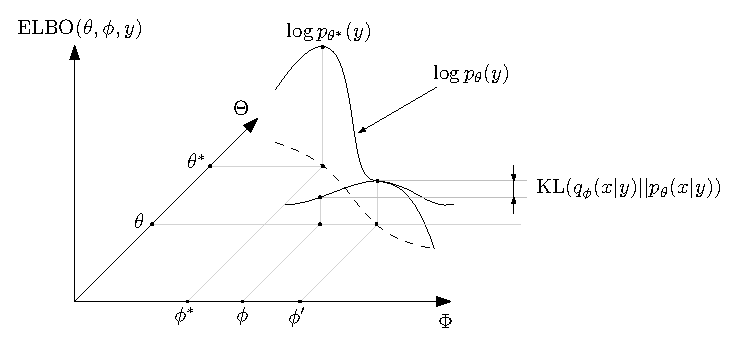
\includegraphics{figures/elbo}
    \caption{Idealized \gls{ELBO} surface.}
    \todo[inline]{How is~\(\theta^*\) different from \(\theta^{\text{true}}\)?}
\end{figure}

\begin{figure}
    \centering
    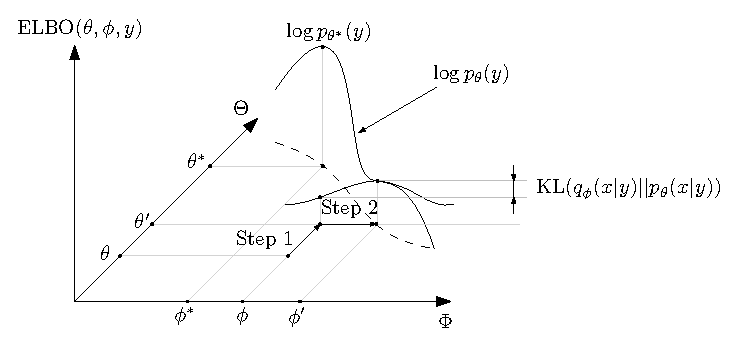
\includegraphics{figures/elbo2}
    \caption{Idealized \gls{ELBO} surface with arrows.}
\end{figure}

\bibliography{notes}
\end{document}

%%% Local Variables:
%%% mode: latex
%%% TeX-master: t
%%% End:
